\documentclass[a4paper,10pt]{article}
\usepackage{paper-ru}
\usepackage{hyperref}
%\usepackage[notref,notcite,color]{showkeys}


\newcommand{\spell}[2]{#1} %for text
%\newcommand{\spell}[2]{#2} %for spelling


\def\thetitle{Землемерная формула}
\def\theauthors{А. Гиль и А. Петрунин}

\hypersetup{colorlinks=true,
citecolor=black,
linkcolor=black,
anchorcolor=black,
filecolor=black,
menucolor=black,
urlcolor=black,
pdftitle={\thetitle},
pdfauthor={\theauthors}
}

%\overfullrule=100mm

\spell{}{\makeatletter\usepackage{environ}\RenewEnviron{figure}[1][]{ [РИС.] }\RenewEnviron{figure*}[1][]{ [РИС.] }\RenewEnviron{wrapfigure}[1][]{ [РИС.] }\usepackage{emptypage}\pagestyle{empty}\makeatother\usepackage[none]{hyphenat}\def\emph{\textit}\def\so{\textit}\renewcommand{\footnote}[1]{\textup{\ (#1)}}\renewcommand{\frac}[2]{(#1)/(#2)}\renewcommand{\tfrac}[2]{(#1)/(#2)}\everydisplay{\textstyle}}


\begin{document}

%\pagestyle{empty}\renewcommand\includegraphics[2][{}]{}


\title{\thetitle}
\author{\theauthors}
\date{}
\maketitle

Землемеры считают площадь четырёхугольника как произведение полусумм противоположных сторон;
то есть, за площадь $S(ABCD)$ четырёхугольника $ABCD$ берут произведение
\[\frac{AB+CD}{2}\cdot \frac{BC+DA}{2}.\]
Эта формла очень древняя; например, она объясняется на глиняной табличке


Эту формулу приводит Брахмагупта в книге «Брахма-спхута-сиддханта» 628 года,
но есть указания, что она применялась гораздо раньше в Египте, Вавилоне и Китае.

В том, что эта формула, вообще говоря, неверна, можно убедиться, рассмотрев следующий рисунок.
\begin{figure}[h!]
\centering
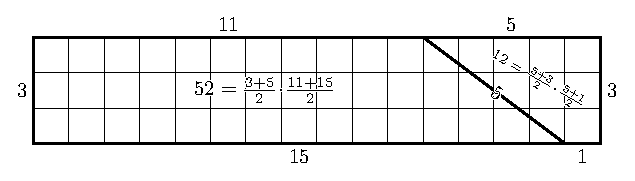
\includegraphics{mpost/pic-10}
\end{figure}
В нём прямоугольник $3\times 16$
разрезан на две трапеции.
Если верить нашей формуле, то площади трапеций равны $52=\tfrac{3+5}2\cdot \tfrac{11+15}2$ и $12=\tfrac{5+3}2\cdot \tfrac{5+1}2$.
Поскольку площадь изначального прямоугольника равна площади $48=3\cdot 16$, часть оказалась больше целого.
В частности, нам удалось разделить прямоугольник на части, увеличив общую площадь.
Смысл понятия «площадь» как раз в том, чтобы запретить подобные махинации, а значит, формула неверна.

(То, что всякому многоугольнику можно приписать значение площади так, чтобы площадь частей равнялась площади целого --- это вовсе не простая теорема; в школьных учебниках геометрии её обычно принимают без доказательства.
Можно, конечно, разбить многоугольник на треугольники, посчитать площадь каждого как половину произведения основания на высоту и сложить результаты.
Однако придётся доказывать, что при другом разбиении результат получится такой же --- в этом и кроется трудность.)

Отметим, что землемерная формула правильно вычисляет площадь прямоугольников;
сейчас мы убедимся, что для всех остальных четырёхугольников формула выдаёт значение выше настоящей площади.

\begin{figure}[ht!]
\centering
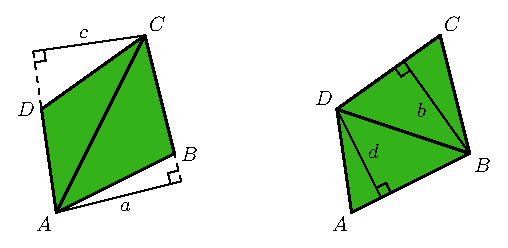
\includegraphics{mpost/pic-20}
\end{figure}

Выпуклый четырёхугольник $ABCD$ можно разбить на треугольники двумя способами, проведя диагональ $AC$ или диагональ $BD$.
Обозначим высоты в этих треугольниках через $a$, $b$, $c$ и $d$, как показано на рисунке.
Так как перпендикуляр короче наклонной, получим
\[AB \ge a,\quad BC\ge b,\quad CD\ge c,\quad DA\ge d.\]
Заметим, что равенства достигаются только если углы $\angle B$, $\angle C$, $\angle D$ и $\angle A$ прямые --- это нам скоро пригодится.

Как известно, площадь треугольника равна половине произведения основания на высоту, поэтому
\begin{align*}
2\cdot S(ABCD)&=S(ABC)+ S(CDA)+S(BCD)+ S(DAC)=
\\
&=\frac {a\cdot BC}2+\frac {c\cdot DA}2+\frac {b\cdot CD}2+\frac {d\cdot AB}2\le
\\
&\le\frac {AB\cdot BC}2+\frac {CD\cdot DA}2+\frac {BC\cdot CD}2+\frac {DA\cdot AB}2=
\\
&=\frac{(AB+CD)\cdot (BC+DA)}{2}.
\end{align*}
Итак, мы показали, что землемерная формула выдаёт значение не меньше, чем настоящая площадь.
Если же достигается равенство, то $AB = a$, $BC = b$, $CD= c$ и $DA= d$.
Как мы уже знаем, это означает, что все углы в четырёхугольнике прямые;
то есть, $ABCD$ --- прямоугольник.

Заметим, что если четырёхугольник $ABCD$ не сильно отличается от прямоугольника, то формула выдаёт очень хорошее приближение.
Например, если каждый из углов $\angle A$, $\angle B$, $\angle C$ и $\angle D$ отличается от прямого не больше чем на $7\degree$ (что весьма ощутимо), то формула ошибётся меньше чем на $1\%$ (это запросто может быть меньше ошибки ваших измерений).
Так что смело пользуйтесь формулой в практических целях и не смейтесь над землемерами.


{\sloppy
\nocite{*}%печатает всё
\printbibliography[heading=bibintoc]
\fussy
}

\end{document}



